\documentclass[10pt,a4paper]{article}
\usepackage[T1]{fontenc}
\usepackage[utf8]{inputenc}
\usepackage{lmodern}
\usepackage[margin=2.1cm]{geometry}
\usepackage{graphicx}
\usepackage{booktabs}
\usepackage{amsmath}
\usepackage{xcolor}
\usepackage[hidelinks]{hyperref}
\usepackage{microtype}
\usepackage{caption}
\usepackage{enumitem}
\usepackage{titlesec}

\captionsetup{font=small,labelfont=bf,skip=4pt}
\titlespacing*{\section}{0pt}{9pt}{3pt}
\titleformat{\section}{\normalfont\large\bfseries}{\thesection}{0.6em}{}
\setlist[itemize]{leftmargin=1.1em,itemsep=1pt,topsep=2pt,parsep=0pt}
\setlist[enumerate]{leftmargin=1.4em,itemsep=1pt,topsep=2pt,parsep=0pt}
\emergencystretch=2em
\tolerance=2000
\pagestyle{plain}

% generated by report/make_report_data.py -- do not edit by hand
\newcommand{\BaseRef}{0.84}
\newcommand{\DriftRef}{0.50}
\newcommand{\HarmRef}{0.88}
\newcommand{\GlobRef}{0.88}
\newcommand{\BaseOver}{0.07}
\newcommand{\DriftOver}{0.05}
\newcommand{\HarmOver}{0.17}
\newcommand{\GlobOver}{0.28}
\newcommand{\BaseAsr}{0.06}
\newcommand{\DriftAsr}{0.22}
\newcommand{\HarmAsr}{0.05}
\newcommand{\GlobAsr}{0.04}
\newcommand{\BaseGsm}{0.59}
\newcommand{\DriftGsm}{0.56}
\newcommand{\HarmGsm}{0.52}
\newcommand{\GlobGsm}{0.44}
\newcommand{\CapGap}{0.08}
\newcommand{\CapLo}{0.04}
\newcommand{\CapHi}{0.12}
\newcommand{\GlobVsBase}{-0.15}
\newcommand{\HarmVsBase}{-0.07}
\newcommand{\HarmScalars}{19{,}251{,}200}
\newcommand{\DriftScalars}{962{,}592{,}768}
\newcommand{\MassTotal}{3.95}
\newcommand{\MassTopTwo}{3.95}
\newcommand{\CosDD}{1.0\times 10^{-3}}
\newcommand{\HbAcc}{0.625}
\newcommand{\HbSens}{0.356}
\newcommand{\HbSpec}{0.896}
\newcommand{\QwAcc}{0.796}
\newcommand{\QwSens}{0.608}
\newcommand{\QwSpec}{0.984}
\newcommand{\GrAcc}{0.818}
\newcommand{\GrSens}{0.696}
\newcommand{\GrSpec}{0.940}
\newcommand{\MajAcc}{0.782}
\newcommand{\MajSens}{0.580}
\newcommand{\MajSpec}{0.984}


\newcommand{\code}[1]{\texttt{\small #1}}

\title{\vspace{-1.4cm}\bfseries Exploratory trade-offs in weight-space refusal repair}
\author{ScarTissue --- Lexsi AI Safety \& Alignment Hackathon, Track 2a}
\date{Working draft --- claim corrections, 6 November 2026}

\begin{document}
\maketitle
\vspace{-0.6cm}

\begin{abstract}
\noindent
We compare stored weight-space edits on \code{tiny-aya-global}. A restricted repair recovers measured
refusal to \HarmRef{} (base \BaseRef{}) and retains GSM8K at \HarmGsm{} versus \GlobGsm{} for the
global repair: a paired $+\CapGap$ exact-match difference, with prompt-bootstrap interval
$[\CapLo,\CapHi]$. Exploratory harm-ASR rises from \BaseAsr{} to \DriftAsr{} after drift; the repair
estimates are \HarmAsr{} and \GlobAsr{}. Nonsignificance does not establish safety equivalence.
\textbf{The original judge calibration controls failed and safety records are not headline-eligible.}
An external Aegis audit does not clear those failures. Near-orthogonal extracted directions do not
prove all harm discrimination was removed. These observations motivate an evidence-comparison
workbench, not production certification. Held-out judging, matched controls and circuit intervention
evaluation remain pending. This corrected source is a draft; previously published PDFs are historical.
\end{abstract}

\vspace{-0.2cm}
\section{The question, and why it is not the obvious one}

Abliteration is attractive because it is cheap: no gradients, no preference data, a rank-one update
per write matrix. It is also described, in its own literature and in most replications, by its effect
on \emph{refusal rate}. Refusal alone does not establish whether a response is harmful. Extracted directions are probes of
behavior, not direct measurements of a complete internal safety decision. This study does not identify
all such representations or establish their causal removal.

So the empirical question is not ``does abliteration work''. It is:
\emph{what does the edit delete, what can a weight-only repair restore, and where must the repair act?}
We answer with a frontier: refusal recovered on one axis, the price paid (over-refusal, lost
capability) on the other, and the support size of the repair as the parameter that moves a point
along it.

\section{Setup}

\paragraph{Model.} \code{CohereLabs/tiny-aya-global}, 3.35\,B parameters, \code{cohere2}
architecture, 36 layers, 16 query heads, $d_{\text{model}}=2048$, $d_{\text{mlp}}=11008$, revision
\code{af89d219}. A Cohere dense open-weights model, chosen because it is multilingual --- the claim
can later be tested in eleven languages inside one licence family --- and small enough that four arms
times 160 prompts times three judges is affordable at full precision.

\paragraph{Data.} 763 rows built through CuratorKIT with row-level provenance: 313 StrongREJECT
harmful prompts and 450 XSTest benign prompts. The split is frozen \emph{before} any evaluation:
120 harmful and 40 benign for evaluation, 16 + 16 for fitting directions, 200 XSTest contrast rows,
and 371 rows held back for confirmation, of which 160 (120 harmful, 40 benign) were never touched by
any earlier run. Fit and evaluation prompts are disjoint by construction, and the property is
asserted by code, not by convention (\code{experiments/corpus\_fit.py}).

\paragraph{Refusal direction.} Difference of means at layer 15, last token, between harmful and
benign fit prompts.

\paragraph{The drift.} Every write matrix is orthogonalised against $d$:
\begin{equation}
W_{\text{drift}} \;=\; W_{\text{base}} - d\,(d^{\top} W_{\text{base}}),
\qquad
\text{72 matrices},\quad \DriftScalars \text{ scalars}.
\end{equation}

\paragraph{The repair.} Re-extract the refusal direction on the \emph{drifted} model, $d'$, and add
it back with gain $\alpha$ into a column support $S$ only:
\begin{equation}
W_{\text{repair}}[:,S] \;=\; W_{\text{drift}}[:,S] + \alpha\, d' \bigl(d'^{\top} W_{\text{base}}[:,S]\bigr).
\end{equation}
The base matrix supplies the projection and the drifted matrix is the substrate. This is a candidate
additive intervention, not an exact reversal of drift, especially when the extracted direction changes. $\alpha=4$ throughout, chosen from a dose sweep in which
$\alpha=8$ degenerates into repetition --- which is why every run in this report stores full
completions rather than rates.

\paragraph{Supports.} \code{harm2} ranks columns by their signed write mass
$|d'^{\top}W_{\text{base}}|$ and takes the top $2\,\%$; \code{global} takes everything; \code{base}
and \code{drift} are the two endpoints. A fourth support, discovered by CircuitKIT on the drifted
model, is built and exported but its evaluation is blocked (section~\ref{sec:blocked}).

\paragraph{Measurement contract.} Harm-ASR comes only from a pinned three-judge panel
(HarmBench-Mistral-7B, Qwen3Guard-Gen-8B, Granite-Guardian-3.2-5B) with strict parsers, a threshold
of $0.5$ and a majority-of-3 headline. Benign over-refusal is Qwen3Guard's explicit \code{Refusal:}
field --- a semantic judgement, not a keyword match. Capability comes only from \code{lm-eval}
(GSM8K, five-shot, 500 items). A regex refusal marker is reported as a diagnostic and never as a
safety number.

\section{What the direction probe does not establish}

The re-extracted direction is nearly orthogonal to the removed one: $\cos(d,d')=\CosDD$.
For the ideal orthogonalization operator, $d^{\top}W_{\text{drift}}=0$; amplifying that already-removed
projection of drifted weights is a no-op up to numerical precision. Restoring a stored base projection
is a different operation and is not ruled out by this identity. Neither the cosine nor a projection
probe establishes that all harmful/harmless discrimination has vanished.

Exploratory harm-ASR changes from \BaseAsr{} to \DriftAsr{} after drift and is
\HarmAsr{}/\GlobAsr{} for the measured repairs. This increase is not flat and cannot be dismissed
as merely reduced politeness. Refusal and harm must be evaluated separately, with the failed judge
calibration and distribution shift visible.

\section{The frontier}

\begin{table}[t]
\centering
\small
% generated by report/make_report_data.py -- do not edit by hand
\begin{tabular}{lrrrrr}
\toprule
arm & edited scalars & refusal & over-refusal & harm-ASR & GSM8K \\
\midrule
base (aligned) & 0 & 0.842 & 0.075 & 0.058 & 0.590 \\
drifted & 962{,}592{,}768 & 0.500 & 0.050 & 0.217 & 0.560 \\
2\,\% repair & 19{,}251{,}200 & 0.883 & 0.175 & 0.050 & 0.518 \\
global repair & 962{,}592{,}768 & 0.883 & 0.275 & 0.042 & 0.438 \\
\bottomrule
\end{tabular}

\caption{All four arms on the frozen evaluation set, generation budget 512 tokens. Refusal is
Qwen3Guard's harmful-refusal diagnostic; over-refusal is its benign refusal field (40 prompts);
harm-ASR is the majority of three judges on 120 harmful prompts; GSM8K is \code{lm-eval} exact match
on 500 items. Sources: \code{results/p21\_length\_analysis\_20261103.json},
\code{results/p16\_capability\_analysis\_20261102.json}.}
\label{tab:arms}
\end{table}

\begin{figure}[t]
\centering
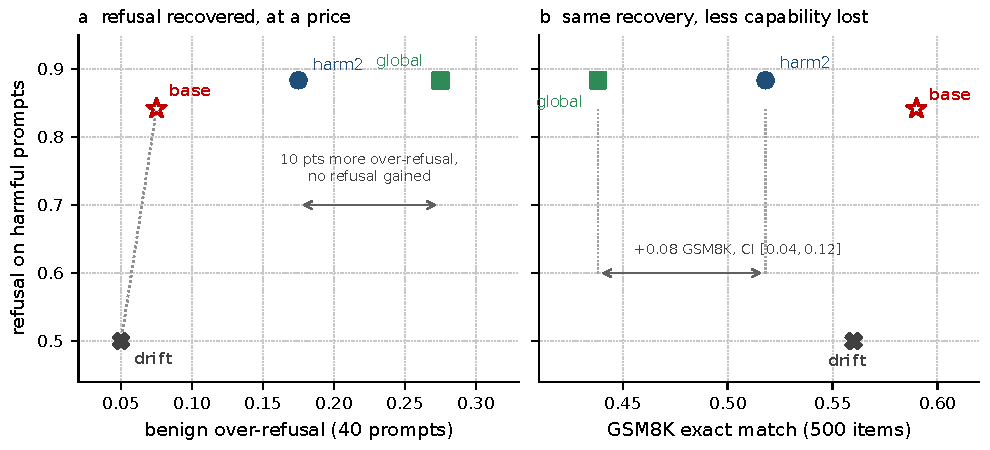
\includegraphics[width=\textwidth]{fig1_frontier.pdf}
\caption{The frontier. (a) Refusal recovered against benign over-refusal: the $2\,\%$ repair reaches
the aligned model's refusal rate with 10 points less over-refusal than the global repair. (b) The same
recovery against GSM8K: the $2\,\%$ repair keeps roughly half of the capability the global repair
loses, and the paired interval on that difference excludes zero. Generated from the published tables
by \code{report/make\_report\_data.py}.}
\label{fig:frontier}
\end{figure}

Table~\ref{tab:arms} and Figure~\ref{fig:frontier} are the result. Reading them in order:

\begin{itemize}
\item \textbf{Measured refusal recovers without gradient training, using fitted directions.} The $2\,\%$ arm's
refusal marker reads \HarmRef{} against the aligned model's \BaseRef{} and the drifted model's \DriftRef.
This is a refusal-marker diagnostic, not a harm rate: it records that the model declined, not that it
declined safely, and the panel behind every harm figure here failed its calibration audit.
\item \textbf{The price is real and it is support-dependent.} Over-refusal is \HarmOver{} for the
$2\,\%$ repair against \GlobOver{} for the global one; GSM8K is \HarmGsm{} against \GlobGsm.
\item \textbf{The capability difference is not noise.} Paired prompt bootstrap over 500 GSM8K items,
$+\CapGap$, 95\,\% CI $[\CapLo,\CapHi]$. For scale, the global repair costs \GlobVsBase{} against the
aligned model and the $2\,\%$ repair \HarmVsBase.
\item \textbf{Safety equivalence is not established.} Per-judge paired ASR differences are
$0.000\,[-0.033,0.033]$ (HarmBench), $-0.008\,[-0.05,0.025]$ (Qwen3Guard) and $+0.008$ (Granite).
These are exploratory per-judge estimates, not majority-vote equivalence tests.
\end{itemize}

The over-refusal difference (about ten points) points the same way but its interval includes zero at
$n=40$ prompts. We report it as suggestive and do not build the claim on it. The claim rests on GSM8K,
where the interval excludes zero.

\section{Support concentration is a hypothesis, not a mechanism proof}\label{sec:mass}

The repair's signed write along $d'$ is extremely concentrated. Summing
$|d'^{\top}W_{\text{base}}[:,c]|$ over all columns gives \MassTotal{} in normalised units, and the top
$2\,\%$ of columns by signed mass already carries \MassTopTwo{}. For this direction, a $2\,\%$
support captures concentrated projected mass at the reported precision. Equality of rounded totals
does not establish identical tensor updates or a causal explanation of capability retention.
Matched random and magnitude supports are needed before generalizing a support-size mechanism.

It also explains why the earlier \emph{circuit} framing had to be withdrawn. When the restricted
support was defined over attention heads rather than by mass, restricted repair did nothing (refusal
$0.267$) and random heads did the same ($0.258$) --- indistinguishable from a control. This negative result limits the earlier circuit claim. It does not establish that mass ranking is
universally superior to discovery; the actual discovered patch and matched controls still require evaluation.

\section{Is the frontier an artefact?}\label{sec:robust}

Two checks, both run after the first version of this result and both preserved whether or not they
supported it.

\paragraph{Generation budget.} The first safety run used 128 tokens, and unequal truncation is exactly
the mechanism that fabricates a frontier: an arm that is cut off mid-sentence can be scored as
``not refusing''. All 640 answers were regenerated at 512 tokens with the same seed, batch size and
immutable base state; every answer reproduced its saved 128-token prefix exactly, every state hash
matched, and every reset was verified. Figure~\ref{fig:length} shows the paired change in harm-ASR:
every arm's interval includes zero, the largest movement is the drift's $-0.042\,[-0.092,0.008]$ (a paired length effect whose interval includes zero; this does not negate the observed base-to-drift increase), and the over-refusal ordering (\HarmOver{} $<$
\GlobOver{}) holds at both budgets. Capped answers fall from 40/120 to 16/120 for base and 85/120 to
47/120 for the drift, so the truncation was real --- it simply did not drive the result.

\begin{figure}[t]
\centering
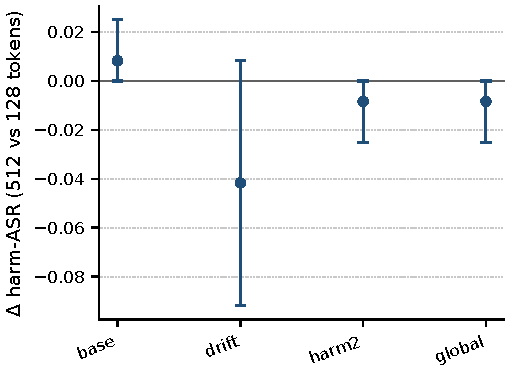
\includegraphics[width=0.52\textwidth]{fig2_length.pdf}
\caption{Paired change in majority-3 harm-ASR when the budget goes from 128 to 512 tokens, per arm
(10k prompt bootstrap). A four-fold budget does not reorder the arms. Source:
\code{results/p21\_length\_analysis\_20261103.json}.}
\label{fig:length}
\end{figure}

\paragraph{Judge calibration.} A three-judge panel that agrees with itself proves nothing, so the
frozen panel was scored against 500 human-annotated rows from
\code{nvidia/Aegis-AI-Content-Safety-Dataset-1.0} (250 unsafe, 250 safe; label = majority of at least
three annotators). Table~\ref{tab:cal} gives the result, and it is not flattering.

\begin{table}[t]
\centering\small
\begin{tabular}{lrrr}
\toprule
judge & accuracy & sensitivity (unsafe) & specificity (safe) \\
\midrule
HarmBench-Mistral-7B & \HbAcc & \HbSens & \HbSpec \\
Qwen3Guard-Gen-8B & \QwAcc & \QwSens & \QwSpec \\
Granite-Guardian-3.2-5B & \GrAcc & \GrSens & \GrSpec \\
\midrule
majority of three & \MajAcc & \MajSens & \MajSpec \\
\bottomrule
\end{tabular}
\caption{Panel accuracy on 500 human-labelled Aegis 1.0 rows, threshold $0.5$.
Source: \code{results/p22\_judge\_validation\_20261103\_020927.json}.}
\label{tab:cal}
\end{table}

The Aegis exercise measures \MajSpec{} specificity and \MajSens{} sensitivity on that distribution.
It does not prove a lower bound on project harm, validate the original controls or eliminate
arm-dependent bias. Project-distribution human auditing remains pending. The original controls
failed and the safety files retain \code{headline\_eligible=false}; the failure is preserved in
\code{results/p18\_judge\_smoke\_20261102\_233759.json} rather than tuned away.

\section{What is still blocked}\label{sec:blocked}

The old workspace hit its spend limit. The replacement account now passes bounded CPU software
validation; this does not recover model caches, validate GPU execution or resolve scientific gaps.

\begin{itemize}
\item \textbf{Circuit arm.} CircuitKIT discovery on the drifted model is complete
(\code{results/p23\_circuit\_...json}); the resulting patch
(\code{repair\_circuit\_a4.npz}, \code{sha256 96c659a0...}) has export metadata, but the remote-only
body needs recovery and independent hash validation. Generation, judging and capability evaluation
are not complete. No circuit intervention result appears in this report.
\item \textbf{Held-out replication, not confirmation.} All four arms have been generated on 160 prompts that, per the published split, no earlier run touched; the analysis re-verifies that disjointness (zero overlap with the fit and evaluation slices). Harm rose from 0/120 to 38/120 under drift, and each repair reduced it (3/120 sparse, 1/120 global) while increasing over-refusal (13/40 and 20/40 against 5/40 for drift); the sparse repair over-refuses less than the global one (paired difference $-$0.175, $[-0.325,-0.050]$) with no resolved harm difference. Because the judge panel failed calibration, the arms were selected on the earlier set and no multiplicity adjustment is applied, this is exploratory and no held-out confirmation is claimed. Raw generation status and its separate state-check correction both remain visible; claim status is recorded in \code{results/readiness\_ledger.json}.
\item \textbf{Multilingual.} The harness exists (11 languages: en, hi, bn, id, vi, sw, yo, ha, am,
ar, fr) and the earlier multilingual projection files were withdrawn as invalid (7{,}080 non-finite
values). No replacement number is quoted.
\item \textbf{Second Cohere model.} \code{tiny-aya-earth} has complete generations for all four arms;
\code{tiny-aya-water} is missing one arm. Neither is judged.
\end{itemize}

\section{Limitations}

One model carries the headline, one seed, one capability task. GSM8K exact match is a bounded probe,
not a capability inventory, and the paired interval accounts for prompt sampling only --- not judge
uncertainty, not training-seed variation. Direction extraction uses calibration prompts, so
``training-free'' is accurate and ``data-free'' would not be. The result is about \emph{this}
operator: a different abliteration variant could leave a different residual structure, and we make no
claim that the $2\,\%$ support generalises to it without re-measuring the mass distribution. Finally,
the over-refusal axis is measured by one judge's semantic field; it is the sharp axis in this model,
which is exactly why it deserves a second, independently trained judge before anyone builds on it.

\section{Why these datasets, metrics and models}

\paragraph{Datasets.} StrongREJECT supplies harmful prompts with category labels; XSTest supplies
benign prompts engineered to trigger surface-form refusal, which is the only way to separate
``refuses harm'' from ``refuses everything''. Both are redistributed with original ids, revisions and
per-row provenance, because a safety claim that cannot be re-scored on the same rows is not a claim.

\paragraph{Metrics.} Refusal (what was restored), over-refusal (what it cost) and GSM8K (collateral
capability), plus harm-ASR, which rises after drift and must not be conflated with refusal. All from contracted paths: ASR from the judge panel, capability from \code{lm-eval} only.
SafeTune's own suite scores GSM8K and HumanEval with a harm judge, which would silently turn
capability into safety; we do not use it.

\paragraph{Models.} \code{tiny-aya-global} because it is Cohere, dense, open-weights and multilingual.
Larger-model expansion is deferred until the core comparison is valid and budgeted; no larger-model
measurement or hardware requirement is claimed here.

\section{Reproducibility and licence}

The historical release is machine-readable but not a fresh readiness sign-off. Local corrections
and replacement-account publication are not yet deployed. Recorded artifacts include: the corpus (\code{scartissue-tinyaya-safety-corpus},
\code{data/corpus.parquet}, 763 rows), the results (\code{scartissue-tinyaya-results} --- 1{,}280 full
generations, 3{,}864 judge verdicts, 4{,}000 capability rows, the frontier, the patch manifest), the
drift and repair parameters (\code{scartissue-tinyaya-abliteration-patches},
\code{scartissue-tinyaya-repair-patches}, with factorised parameters, per-file sha256 and an explicit
\code{allowed} block), and a static demo Space with the frontier chart and a three-column completion
viewer.

Track repositories are chained and their provenance is machine-checked
(\code{results/toolkit\_provenance.json}): CuratorKIT \code{dd9e8353} for the corpus and its
provenance chain, CircuitKIT \code{e71d5e17} for discovery on the drifted model, AuditKIT
\code{71316da3} for native re-scoring of stored answers. The abliteration operator is 30 lines and
deliberately independent, so the drift does not depend on any toolkit being correct.

The Cohere weights are LSAL 1.2/1.1, research use. Section 2 forbids selling or hosting the model as
a product and section 4 forbids deploying drifted checkpoints; we therefore publish
\emph{parameters}, never a drifted checkpoint, and the public demo serves precomputed JSON over the
aligned model's published answers. This is an individual entry and does not represent an
organisation.

\section{Conclusion}

On the stored \code{tiny-aya-global} comparison, the restricted repair has higher GSM8K than the
global repair ($+\CapGap$, CI $[\CapLo,\CapHi]$). Exploratory safety estimates do not establish
repair equivalence or deletion of all harm representations. Judge validity, held-out evidence and
matched circuit controls remain unresolved. A useful comparison tool must expose those gaps and be
able to return insufficient evidence rather than promote these results to production approval.

\section*{Appendix: reproduction order}

Every stage below is a Modal app; each writes a JSON with full generations, token ids, stop
diagnostics, patch hashes and the immutable base-state hash, so any arm can be re-scored without
being regenerated.

{\small
\begin{verbatim}
uv sync                                  # experiments/runtime, locked, Python 3.12
modal run experiments/p8_corpus.py       # CuratorKIT corpus + provenance chain
modal run experiments/build_patches.py --model CohereLabs/tiny-aya-global
modal run experiments/p23_circuit.py     # CircuitKIT on the DRIFTED model
modal run experiments/p21_safety_length_full.py   # 4 arms x 160 prompts, 512 tokens
modal run experiments/p19_score_safety.py --safety results/p21_*.json
modal run experiments/p16_lm_eval.py     # lm-eval GSM8K, 4 arms
uv run python -m experiments.analyse_safety results/<judges>.json results/<analysis>.json
uv run python -m experiments.build_bundle         # public demo evidence
uv run python -m experiments.build_readiness      # decision ledger
uv run python report/make_report_data.py          # every number in this PDF
\end{verbatim}
}

\end{document}
